% $HeadURL: https://sbgn.svn.sourceforge.net/svnroot/sbgn/ProcessDiagram/tags/L1V1.3Full/sources/necessary_stim.tex $

%%%%%%%%%%%%%%%%%%%%%%%%%%%%%%%%%%%%%%%%%%%%%%%%%%%%%%%%%%%%%%%%%%%%%%
%%                     Necessary_Stim
%%%%%%%%%%%%%%%%%%%%%%%%%%%%%%%%%%%%%%%%%%%%%%%%%%%%%%%%%%%%%%%%%%%%%%

\subsection{Glyph: \glyph{Necessary stimulation}}\label{sec:necessary_stim}

A necessary stimulation, is one that is necessary for a process to take place. A process modulated by a necessary stimulation can only occur when this necessary stimulation is active. The target extremity of a \glyph{necessary stimulation} carries an open arrow (to remind that it is a \glyph{stimulation}) coming after a larger vertical bar.

\begin{figure}[H]
  \centering
  \includegraphics[scale = 0.5]{images/necessary_stim}
  \caption{The \PD glyph for \glyph{Necessary Stimulation}.}
  \label{fig:Necessary Stimulation}
\end{figure}
